\subsubsection{Ganache} \label{subsection:4-2-3-2-ganache}

\logo{chapter-4/4.2.ganache-logo}{Ganache logo}

Το Ganache\footnote{\url{https://trufflesuite.com/ganache/}} είναι ένα λογισμικό που παρέχει ένα βοηθητικό προσωπικό Ethereum blockchain για ταχεία ανάπτυξη αποκεντρωμένων εφαρμογών και αποτελεί επίσης τμήμα της σουίτας Truffle. Διατίθεται τόσο ως desktop εφαρμογή με UI, όσο και ως CLI (command-line interface).

To Ganache παρέχει ισχυρά εργαλεία για την ανάπτυξη έξυπνων συμβολαίων, όπως:
\begin{itemize}
	\item Block explorer, μέσω του οποίου μπορούν να εξεταστούν λεπτομερώς όλα τα blocks και οι συναλλαγές που έλαβαν χώρα.
	\item Εξρεύνηση των εσωτερικών των contracts και των πυροδοτημένων event τους.
	\item Ενδελεχές αρχείο καταγραφής της εξόδου του blockchain, το οποίο περιλαμβάνει σημαντικές πληροφορίες για τον εντοπισμό σφαλμάτων.
	\item Δυνατότητα διαμόρφωσης του χρόνου εξόρυξης των block, έτσι ώστε να αρμόζει με τις εκάστοτε ανάγκες (αυτόματη εξόρυξη ή εξόρυξη σε προσαρμοσμένο χρονικό διάστημα).
\end{itemize}

\begin{figure}[H]
	\centering
	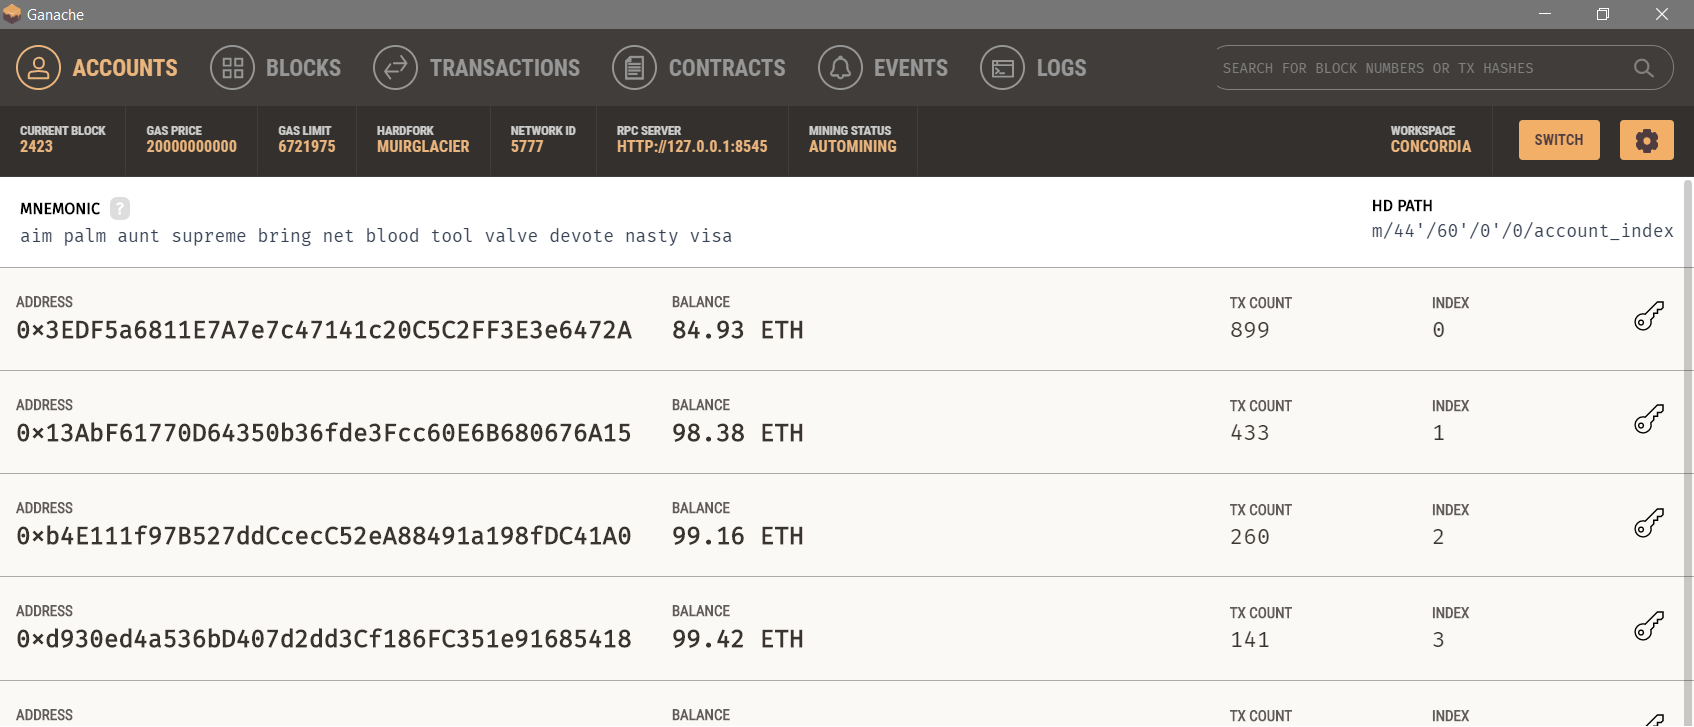
\includegraphics[width=.95\textwidth]{assets/figures/chapter-4/4.2.ganache-gui}
	\caption{Ganache (desktop εφαρμογή)}
\end{figure}

Το Ganache έχει το αποθετήριό του στο GitHub (\url{https://github.com/trufflesuite/ganache}) και διατίθεται μέσω του μητρώου npm (\url{https://www.npmjs.com/package/ganache}).